\documentclass[12pt]{article}
\usepackage[paper=letterpaper,margin=1.5cm]{geometry}
\usepackage{amsmath}
\usepackage{amssymb}
\usepackage{amsfonts}
\usepackage{mathtools}
%\usepackage[utf8]{inputenc}
%\usepackage{newtxtext, newtxmath}
\usepackage{lmodern}     % set math font to Latin modern math
\usepackage[T1]{fontenc}
\renewcommand\rmdefault{ptm}
%\usepackage{enumitem}
\usepackage[shortlabels]{enumitem}
\usepackage{titling}
\usepackage{graphicx}
\usepackage[colorlinks=true]{hyperref}
\usepackage{setspace}
\usepackage{subfigure} 
\usepackage{braket}
\usepackage{color}
\usepackage{tabularx}
\usepackage[table]{xcolor}
\usepackage{listings}
\usepackage{mathrsfs}
\usepackage{stackengine}
\usepackage{physics}
\usepackage{afterpage}
\usepackage{pdfpages}
\usepackage[export]{adjustbox}
\usepackage{biblatex}

\setstackEOL{\\}

\definecolor{dkgreen}{rgb}{0,0.6,0}
\definecolor{gray}{rgb}{0.5,0.5,0.5}
\definecolor{mauve}{rgb}{0.58,0,0.82}


\lstset{frame=tb,
  language=Python,
  aboveskip=3mm,
  belowskip=3mm,
  showstringspaces=false,
  columns=flexible,
  basicstyle={\small\ttfamily},
  numbers=none,
  numberstyle=\tiny\color{gray},
  keywordstyle=\color{blue},
  commentstyle=\color{dkgreen},
  stringstyle=\color{mauve},
  breaklines=true,
  breakatwhitespace=true,
  tabsize=3
}
\setlength{\droptitle}{-6em}

\makeatletter
% we use \prefix@<level> only if it is defined
\renewcommand{\@seccntformat}[1]{%
  \ifcsname prefix@#1\endcsname
    \csname prefix@#1\endcsname
  \else
    \csname the#1\endcsname\quad
  \fi}
% define \prefix@section
\newcommand\prefix@section{}
\newcommand{\prefix@subsection}{}
\newcommand{\prefix@subsubsection}{}
\renewcommand{\thesubsection}{\arabic{subsection}}
\makeatother
\DeclareMathOperator*{\argmin}{argmin}
\newcommand{\partbreak}{\begin{center}\rule{17.5cm}{2pt}\end{center}}
\newcommand{\alignbreak}{\begin{center}\rule{15cm}{1pt}\end{center}}
\newcommand{\tightalignbreak}{\vspace{-5mm}\alignbreak\vspace{-5mm}}
\newcommand{\hop}{\vspace{1mm}}
\newcommand{\jump}{\vspace{5mm}}
\newcommand{\R}{\mathbb{R}}
\newcommand{\C}{\mathbb{C}}
\newcommand{\N}{\mathbb{N}}
\newcommand{\G}{\mathbb{G}}
\renewcommand{\S}{\mathbb{S}}
\newcommand{\bt}{\textbf}
\newcommand{\xdot}{\dot{x}}
\renewcommand{\star}{^{*}}
\newcommand{\ydot}{\dot{y}}
\newcommand{\lm}{\mathrm{\lambda}}
\renewcommand{\th}{\theta}
\newcommand{\id}{\mathbb{I}}
\newcommand{\si}{\Sigma}
\newcommand{\Si}{\si}
\newcommand{\inv}{^{-1}}
\newcommand{\T}{^\intercal}
\renewcommand{\tr}{\text{tr}}
\newcommand{\ep}{\varepsilon}
\newcommand{\ph}{\varphi}
%\renewcomand{\norm}[1]{\left\lVert#1\right\rVert}
\definecolor{cit}{rgb}{0.05,0.2,0.45}
\addtolength{\jot}{1em}
\newcommand{\solution}[1]{

\noindent{\color{cit}\textbf{Solution:} #1}}

\newcounter{tmpctr}
\newcommand\fancyRoman[1]{%
  \setcounter{tmpctr}{#1}%
  \setbox0=\hbox{\kern0.3pt\textsf{\Roman{tmpctr}}}%
  \setstackgap{S}{-.9pt}%
  \Shortstack{\rule{\dimexpr\wd0+.1ex}{.9pt}\\\copy0\\
              \rule{\dimexpr\wd0+.1ex}{.9pt}}%
}

\newcommand{\Id}{\fancyRoman{2}}

% Enter the specific assignment number and topic of that assignment below, and replace "Your Name" with your actual name.
\title{STAT 31020: Homework 3}
\author{Caleb Derrickson}
\date{January 24, 2024}

\begin{document}
\onehalfspacing
\maketitle
\allowdisplaybreaks
\tableofcontents

\newpage
\section{Problem 1}
Let $f(x): \R^n \rightarrow \R$ be a three times continuously differentiable function and $x\star$ a local minimum of $f(x)$ that satisfies the sufficient second order-conditions. Consider the iteration
\begin{align}
    x_{k+1} = x_k - \left(\grad^2_{xx}f(x_k) + \norm{\grad_x f(x_k)}^p \ \id_n \right)\inv \grad f(x_k).\label{p1: first}
\end{align}
Here, $p > 0$ and $\id_n$ is the identity matrix of order $n$. Assume that you know that $x_k \rightarrow x\star$.
\subsection{Problem 1, part 1}
Show that the sequence $x_k$ converges to $x\star$ faster than superlinearly.
\partbreak
\begin{solution}

    This will be given as a consequence to the next part. 
\end{solution}
\subsection{Problem 1, part 2}
Determine the largest value $q$ such that 
\[\limsup \frac{\norm{x_{k+1} - x\star}}{\norm{x_k - x\star}^q} < \infty\] 
as a function of $p$ for $p > 0$.
\partbreak
\begin{solution}

    I will break this derivation up into sections dedicated to simple steps (which will be bundled together) and other sections which describe a particular step in more detail Note that I will be occasionally short-handing arguments of functions (such as $\grad f(x_k)$ into $\grad f_k$) to condense lines. We first start by adding a $-x\star$ to both sides of \ref{p1: first}. 
    \[\implies x_{k+1} - x\star = x_k - x\star - (\grad^2f_k + \norm{\grad f_k}^p\id_n)\inv \grad f_k.\]
    We will then group up terms by bringing out the inverted matrix on the left hand side.
    \[\implies x_{k+1} - x\star = \left ( \grad^2f_k + \norm{\grad f_k}^p \id_n\right)\inv\left[ \left(\grad^2f_k + \norm{\grad f_k}^p \id_n\right)(x_k - x\star) - \grad f_k\right]\]
    Next, define a helper function $\psi$ as $\psi(t) = \grad f(x\star + t(x_k - x\star))$. Note that $\psi(1) = \grad f_k$ and $\psi(0) = \grad f(x\star)$. Since $x\star$ is a strict local minimum of $f$, $\grad f(x\star) = 0$, so we can include this in whenever we wish. We can therefore say that $\grad f_k = \psi(1) - \psi(0)$, which by the Fundamental Theorem of Calculus,\footnote{This is well defined since the derivative of $\psi(t)$ is well defined. } 
    \[\grad f_k = \psi(1) - \psi(0) =\int_0^1 \psi '(t) \ dt = \int_0^1 \grad^2 f(x\star + t(x_k - x\star)) (x_k - x\star) \ dt.\]
    We will then do some intermediate steps below.
{\footnotesize
    \begin{align*}
        x_{k+1} - x\star &= \left ( \grad^2f_k + \norm{\grad f_k}^p \id_n\right)\inv\left[ \left(\grad^2f_k + \norm{\grad f_k}^p \id_n\right)(x_k - x\star) - \grad f_k\right] \\
         &= \left ( \grad^2f_k + \norm{\grad f_k}^p \id_n\right)\inv\left[ \left(\grad^2f_k + \norm{\grad f_k}^p \id_n\right)(x_k - x\star) - \int_0^1 \grad^2 f(x\star + t(x_k - x\star)) (x_k - x\star) \ dt\right]\\ 
         &= \left ( \grad^2f_k + \norm{\grad f_k}^p \id_n\right)\inv\left[ \int_0^1 \left[ \grad^2 f_k - \grad^2f(x\star + t(x_k - x\star)) + \norm{\grad f_k}^p\right](x_k - x\star) \ dt\right]\\ 
    \end{align*}}
    \vspace{-20mm}
    
    The steps above were just some simple rearranging and adding in the helper function. We can then take norms on both sides to get
    \begin{align}
        \norm{x_{k+1} - x\star} = \norm{\left ( \grad^2f_k + \norm{\grad f_k}^p \id_n\right)\inv\left[ \int_0^1 \left[ \grad^2 f_k - \grad^2f(x\star + t(x_k - x\star)) + \norm{\grad f_k}^p\right](x_k - x\star) \ dt\right]}.\label{p1:star}
    \end{align}
    From here we will be taking advantage of three notable things:
    \begin{enumerate}[(a)]
        \item We wish to find an upper bound to $\norm{\left ( \grad^2f_k + \norm{\grad f_k}^p \id_n\right)\inv}$. Note that for any neighborhood of the local minimum $x\star$, $\lm_{\min}(\grad^2f(x)) \geq \frac{1}{2} \lm_{\min}(\grad^2f(x\star))$ for any $x$ in that neighborhood. Furthermore, we can take $\left( \grad^2f_k + \norm{\grad f_k}^p \id_n\right)\inv \succ 0$, since its inverse is positive definite.\footnote{Or within the region such that It can be bounded below by $\grad^2f(x\star)$, which is positive definite by the second sufficient condition.} The norm of this matrix is then its largest eigenvalue (assuming we're in the $2$ norm). So that
        \[\norm{\left( \grad^2f_k + \norm{\grad f_k}^p \id_n\right)\inv} = \frac{1}{\lm_{\min}(\grad^2f_k) + \norm{\grad f_k}^p}.\]
        We can then again bound this ratio by removing the additional term, to get 
        \[\norm{\left( \grad^2f_k + \norm{\grad f_k}^p \id_n\right)\inv} \leq \frac{1}{\lm_{\min}(\grad^2 f_k)}.\]
        By the argument above, this can then be bounded again to get
        \[\norm{\left( \grad^2f_k + \norm{\grad f_k}^p \id_n\right)\inv} \leq \frac{2}{\lm_{\min}(\grad^2f_k)} = 2\norm{\grad^2f(x\star)\inv}.\]
        \item We can note that 
        \[\norm{\int \psi \ dt} \leq \int \norm{\psi} \ dt\]
        for any integrable function $\psi$. 
        \item We will take the norm to be consistent. That is, for a matrix $A$ and suitable vector $b$, $\norm{Ab} \leq \norm{A}\norm{b}$.
    \end{enumerate}
    
    \newpage
    We will then apply $(c)$ to \ref{p1:star} to get 
    \[\norm{x_{k+1} - x\star} \leq \norm{\left ( \grad^2f_k + \norm{\grad f_k}^p \id_n\right)\inv}\norm{\left[ \int_0^1 \left[ \grad^2 f_k - \grad^2f(x\star + t(x_k - x\star)) + \norm{\grad f_k}^p\id_n\right](x_k - x\star) \ dt\right]}.\]
    Then, applying $(a)$ and $(b)$, 
    \[\norm{x_{k+1} - x\star} \leq 2\norm{\grad^2f(x\star)\inv} \int_0^1 \left[ \norm{\grad^2 f_k - \grad^2f(x\star + t(x_k - x\star)) + \norm{\grad f_k}^p\id_n}\norm{(x_k - x\star)} \right] \ dt.\]
    We can then successively bound $\norm{x_{k+1} - x\star}$ via the following steps.
    \begin{align*}
        \norm{x_{k+1} - x\star} &\leq 2\norm{\grad^2f(x\star)\inv}\int_0^1 \left[ \norm{\grad^2f_k + \norm{\grad f_k}^p\id_n - \grad^2 f(x\star + t(x_k - x\star))}\right]\norm{x_k - x\star} \ dt \\
        &\leq 2\norm{\grad^2f(x\star)\inv}\int_0^1 \left[ \norm{\grad^2f_k - \grad^2 f(x\star + t(x_k - x\star))}  + \norm{\grad f_k}^p\right]\norm{x_k - x\star} \ dt \\
        &\leq 2\norm{\grad^2f(x\star)\inv}\int_0^1 \left[ L(1 - t)\norm{x_k - x\star}  + \norm{\grad f_k}^p\right]\norm{x_k - x\star} \ dt \\
        &= 2\norm{\grad^2f(x\star)\inv}\left[ \frac{L}{2}\norm{x_k - x\star}^2  + \norm{\grad f_k}^p\norm{x_k - x\star}\right] \\
        &= 2\norm{\grad^2f(x\star)\inv}\left[ \frac{L}{2}\norm{x_k - x\star}^2  + \norm{\grad f(x_k) - \grad f(x\star)}^p\norm{x_k - x\star}\right] \\
        &\leq 2\norm{\grad^2f(x\star)\inv}\left[ \frac{L}{2}\norm{x_k - x\star}^2  + (L')^p\norm{x_k - x\star}^{(1+p)}\right] \\
        &=  L\norm{\grad^2f(x\star)\inv}\norm{x_k - x\star}^2  + 2(L')^p\norm{\grad^2f(x\star)\inv}\norm{x_k - x\star}^{(1+p)}
    \end{align*}
    Note that $\grad^2 f$ is deferentially continuous and its derivative is bounded, thus $\grad^2 f$ is continuously Lipschitz. This holds as well for $\grad f$. Denote their Lipschitz constants as $L$ and $L'$, respectively. To group the terms together, define a constant $C = \max \{ L, 2(L')^p\}$. We then get
    \[\norm{x_{k+1} - x\star} \leq C\norm{\grad^2f(x\star)\inv}\left[ \norm{x_k - x\star}^2 + \norm{x_k - x\star}^{(1 + p)}\right].\]
    
    \newpage
    This gives us a fair enough bound for lower values of $k$, but for sufficiently large $k$, we will see one of these terms dominate. In particular, we will see the term which is raised by the least exponent to dominate. Thus, we can effectively ignore the term being raised to the larger power for sufficiently large $k$. \footnote{This can also be interpreted as taking the limsup of the function.} If we define $q = \min \{ 2, 1 + p \}$, then we can see that 
    \[\frac{\norm{x_{k+1} - x\star}}{\norm{x_k - x\star}^q} \leq C\norm{\grad^2f(x\star)\inv}\]
    for all $k$. Then taking the limit as $k$ goes to $\infty$, we see that this ratio is bounded above by some constant. Thus, the iteration converges faster than superlinearly for any value $p > 0$ (satisfying part 1), and the largest $q$ value is 2.
\end{solution}

\newpage
\subsection{Problem 1, part 3}
Repeat now the problem for the iteration
\[x_{k+1} = x_k - \left( \grad^2_{xx}f(x_k) + \grad f(x_k) \grad f(x_k)\T + \norm{\grad_x f(x_k)}^p \id_n\right)\inv \grad f(x_k)\]
\partbreak
\begin{solution}

    This is almost the same derivation as above. I will stop when something is meaningfully changed below.
{\footnotesize
    \begin{align*}
        &x_{k+1} = x_k - \left( \grad^2_{xx}f(x_k) + \grad f(x_k) \grad f(x_k)\T + \norm{\grad_x f(x_k)}^p \id_n\right)\inv \grad f(x_k)\\
        &x_{k+1} - x\star = x_k -x\star - \left( \grad^2_{xx}f(x_k) + \grad f(x_k) \grad f(x_k)\T + \norm{\grad_x f(x_k)}^p \id_n\right)\inv \grad f(x_k)\\
        &= \left( \grad^2_{xx}f(x_k) + \grad f(x_k) \grad f(x_k)\T + \norm{\grad_x f(x_k)}^p \id_n\right)\inv \left[\left( \grad^2_{xx}f(x_k) + \grad f(x_k) \grad f(x_k)\T + \norm{\grad_x f(x_k)}^p \id_n\right)(x_k -x\star) - \grad f(x_k)\right]\\
        &= \left( A\right)\inv \left[\left( \grad^2_{xx}f(x_k) + \grad f(x_k) \grad f(x_k)\T + \norm{\grad_x f(x_k)}^p \id_n\right)(x_k -x\star) - \int_0^1\grad^2 f(x\star + t(x_k - x\star))(x_k - x\star) \ dt\right]\\
        &= \left( A\right)\inv \left[ \int_0^1 \left( \grad^2_{xx}f(x_k) + \grad f(x_k) \grad f(x_k)\T + \norm{\grad_x f(x_k)}^p \id_n + \grad^2 f(x\star + t(x_k - x\star))\right)(x_k - x\star) \ dt\right]\\
        &\implies \norm{x_{k+1} - x\star}=\\
        &\norm{\left( A\right)\inv \left[ \int_0^1 \left( \grad^2_{xx}f(x_k) + \grad f(x_k) \grad f(x_k)\T + \norm{\grad_x f(x_k)}^p \id_n + \grad^2 f(x\star + t(x_k - x\star))\right)(x_k - x\star) \ dt\right]}\\
        &\leq \norm{A\inv} \int_0^1 \left[ \norm{\grad^2f(x_k) - \grad^2f(x\star + t(x_k - x\star))} + \norm{\grad f_k \grad f_k\T} + \norm{\grad f_k}^p \ dt \right]\norm{x_k - x\star}\\
        &\leq \norm{A\inv} \int_0^1 \left[ L \norm{x_k - x\star}(1 - t) + \norm{\grad f_k }\norm{\grad f_k } + \norm{\grad f_k}^p \ dt \right]\norm{x_k - x\star}\\
        &\leq \norm{A\inv}  \left[ \frac{L}{2} \norm{x_k - x\star} + \norm{\grad f_k}^2 + \norm{\grad f_k}^p\right]\norm{x_k - x\star}\\
        &= \norm{A\inv}  \left[ \frac{L}{2} \norm{x_k - x\star} + \norm{\grad f(x_k) - \grad f(x\star)}^2 + \norm{\grad f(x_k) - \grad f(x\star)}^p\right]\norm{x_k - x\star}\\
        &\leq \norm{A\inv}  \left[ \frac{L}{2} \norm{x_k - x\star} + (L')^2\norm{x_k - x\star}^2 + (L')^p\norm{x_k - x\star}^p\right]\norm{x_k - x\star}\\
        &= \norm{A\inv}  \left[ \frac{L}{2} \norm{x_k - x\star}^2 + (L')^2\norm{x_k - x\star}^3 + (L')^p\norm{x_k - x\star}^{(1+p)}\right]\\ 
    \end{align*}
}
    \newpage
    The derivation requires more than the width of the page to write in its entirety. Because of this, I substituted $A$ as the inverted norm on the left of the integral. This term will be considered below. By the same reasoning from the previous part, we will take
    \[\norm{A\inv} = \frac{1}{\lm_{\min}(\grad^2f_k) + \lm_{\min} (\grad f_k \grad f_k\T ) + \norm{\grad f_k}^p}.\]
    This \textit{might} not be the correct interpretation or the max eigenvalue of $\norm{A\inv}$, because It might not be the case that we are taking the smallest eigenvalues of both matrices. Either way, it doesn't matter since we will bound it like we did in the last part. Note that $\grad f_k \grad f_k\T$ is a rank one matrix, so its minimum eigenvalue is zero \footnote{If we are in two dimensions or higher.}, so this can be rewritten as 
    \[\norm{A\inv} = \frac{1}{\lm_{\min}(\grad^2f_k) + \norm{\grad f_k}^p}.\]
    This is the same as in the last part, which we found to be bounded by $2\norm{\grad f(x\star)\inv}$. Substituting this in, we get
    \[\norm{x_{k+1} - x\star} \leq \norm{\grad f(x\star)\inv} \left[ L \norm{x_k - x\star}^2 + 2(L')^2\norm{x_k - x\star}^3 + 2(L')^p\norm{x_k - x\star}^{(1+p)}\right].\]
    Take $C = \max \{ L, 2(L')^2, 2(L')^p \}$. Then,
    \[\norm{x_{k+1} - x\star} \leq \norm{\grad f(x\star)\inv} C\left[ \norm{x_k - x\star}^2 + \norm{x_k - x\star}^3 + \norm{x_k - x\star}^{(1+p)}\right].\]
    This will again be dominated by the least power term, so take $q = \min \{ 2, 3, 1 + p\} = \min \{ 2, 1 + p\}$. Note that $p > 0$, so the limit as $k$ goes to $\infty$ is zero, which means the sequence converges more than superlinearly. The fastest it can converge is superquadratically, or when $q = 2$.
\end{solution}

\newpage
\section{Problem 2}
I will try to "walk you" through a justification for the equations 4.8 in Theorem 4.1 that we will use when we characterize the solution of the trust region problem. The approach I used can be used to prove the optimality conditions for constrained optimization, using the barrier method- which is intrinsic to a class of algorithms called interior point methods. 

\jump
Under the conditions of Theorem 4.1 in the 2013 (?) textbook edition, consider the problem $ \\ \min_{p \in \R^n} m(p, \mu) := m(p) - \mu \log (\Delta^2 - p\T p),$ where $m(p) := f + g\T p + \frac{1}{2}p\T Bp$ is a quadratic function model. Observe that the domain of $m(p, \mu)$ is the interior of the trust region.
\subsection{Problem 2, part a}
Show that, for any $0 < \mu \leq 1$, you have that $m(p, \mu)$ is bounded below in its domain, uniformly with respect to $\mu$.
\partbreak
\begin{solution}

    Note the domain of $m(p, \mu)$ is restricted on the values taken by $\Delta ^2 - p\T p$. In particular, since we don't want the log to blow up, we want $\Delta^2 - p\T p > 0$, in particular, we want $\norm{p} < \Delta$. FINISH THIS ONE.
\end{solution}

\newpage
\subsection{Problem 2, part b}
Conclude that $m(p, \mu)$ must have a global minimum. denote that point by $p(\mu)$ if there is more than one such point, choose one of them at random.
\partbreak
\begin{solution}
    
    Since $p(p, \mu)$ is bounded below on its domain, we have that there must be some finite minimum value of $m$ achieved by some $p\star$. Since the additional log term is strictly increasing, this would not affect the number of minimums achieved by the function $m(p)$. Since $m(p)$ is given as convex, there is only one global minimum, which we will denote by $p\star$. Therefore, the global minimum is unique. 
\end{solution}
\subsection{Problem 2, part c}
Prove the following lemma: If A is a matrix of full column rank, then $b = A\lm \implies \norm{\lm} \leq \frac{\norm{b}}{\si_m}$, where $\sigma_m$ is the smallest singular value of A, and the norms used are 2 norms.
\partbreak
\begin{solution}

    By consistency of the 2-norm, we have that $\norm{A\lm}_2 \leq \norm{A}_2\norm{\lm}_2$. Thus $\norm{b}_2 = \norm{A\lm}_2 \leq \norm{A}_2 \norm{\lm}_2$. This implies $\norm{\lm}_2 \leq \frac{\norm{b}_2}{\norm{A}_2}$. Note that $\norm{A}_2$ is the largest singular value of $A$, which has reciprocal less than or equal to the smallest singular value (assuming it is nonzero). Therefore,  $\norm{\lm}_2 \leq \frac{\norm{b}_2}{\sigma_m}$, which is what we wanted. 
\end{solution}
\subsection{Problem 2, part d}
Conclude that, when writing the optimality conditions of the problem stated, you must have $\grad_p m(p) + \lm(\mu)p = 0$ at the global minimum. Use part $(c)$ to chow that $\lm(\mu)$ must be uniformly bounded in $\mu$ (above).
\partbreak
\begin{solution}

    By the first optimality condition, $\lm(\mu)p = -g - Bp$. By taking the gradient of $m(p)$, we can see that the right hand side is equal to $-\grad_p m(p)$. Then $\lm(\mu)p = -\grad_p m(p)$. Therefore, $\lm(\mu)p + \grad_p m(p)= 0$. To show that $\lm$ is bounded above, we take norms on the first optimality condition, and rewrite it in the same form as in part $(c)$ to get
    \[\norm{p} \leq \frac{\norm{g}}{\sigma_{m}(B + \lm(\mu)\id )}\]
    By the third optimality condition, we have that the matrix $B + \lm(\mu)\id$ is positive semidefinite. If the smallest singular value is zero, then we have a problem. So we will just look at the case when the smallest singular value is not zero. Note that $\lm \geq 0$, so when evaluating the smallest singular value of $B + \lm \id$, we can look at them individually. This means
    \[\norm{p} \leq \frac{\norm{g}}{\sigma_{m}(B) + \lm(\mu) }\]
    Then rearranging for $\lm$, we get
    \[\lm(\mu) \leq \frac{\norm{g}}{\norm{p}}\]
    So $\lm$ is bounded above. Note that if $\norm{p} = 0$, then $\grad_p m(p = 0) + 0 = 0$. This means the gradient is zero, which is a contradiction.
\end{solution}



\newpage
\section{Problem 3}
\subsection{Problem 3, parts 1 - 3}
\begin{enumerate}
    \item Implement Newton's method with Hessian modification (which I will call NMHM)  - Algorithm 3.2; with the matrix $E_k$ computed by Algorithm 3.3 - and backtracking line search (you can reuse the code from last homework if you did good encapsulation). Allow the number of iterations to be a parameter.
    \item Also implement the vanilla Newton (which I will call VN) algorithm, that is\\
    $x_{k+1} = x_k - (\grad^2_{xx}f(x_k))\inv \grad f(x_k)$\\
    As pointed out in class, it could fail to find a new iterate if the Hessian is singular, bit in the circumstances I will ask you to run it it should not. 
    \item You will apply the method to the following function (Fenton's Function); \\
    $f(x_1, x_2) = \frac{1}{10}\left ( 12 + x_1^2 + \frac{1 + x_2^2}{x_1^2} + \frac{x_1^2x_2^2 + 100}{(x_1x_2)^4}\right)$\\
    If you code the derivatives by hand, then implement the function (in Matlab) [f, g, H] = fentonfgH(x), where x is the point of function gradient, and Hessian evaluation.
\end{enumerate}
\partbreak
\begin{solution}

    I am grouping these all together since they ask for no results - just to implement the methods on Fenton's Function. Needless to say I have done so, and can be seen in my GitHub folder. I've tried my best at abstracting away the function being minimized for more flexible code, though I am fairly new to Matlab. 
\end{solution}

\newpage
\subsection{Problem 3, part 4}
Run NMHM and VN on Fenton's Function and compare the results as follows:
\begin{itemize}[a.]
    \item First, initialize both methods at x = [3, 2].
    \item Second, initialize both methods at x = [3, 4].
\end{itemize}
Explain what you observe and how or why does it occur. Compare the methods in iteration counts and general outcome.
\partbreak
\begin{solution}

    I have given the individual plots for convergence with respect to initial condition [3, 2] first, then [3, 4] second. I tried my best to make it look as legible as possible - adding two colorbars on the combined figures was a pain. It seems that the Modified Newton is either bugged an is not converging to the correct point, or that the first initial step "jumped" it into another well. I'm not entirely sure which one is the case. I have tweaked so many things in my code to see what happens, but in any other configuration the Modified Newton diverges. The number of iterations in each step is also interesting, as we see the Modified Newton gradually converging to the minimum, whereas the Vanilla Newton takes 8 times fewer iterations, but seems far less stable. Once surprising thing to note for Figure \ref{fig:NMHM42} is that we see convergence for the Modified Newton in the initial condition [3, 4], whereas the Vanilla Newton diverges.   
\end{solution}

\newpage
\begin{figure*}[!htb]
  \centering
  \begin{minipage}{0.45\textwidth}
    \centering
    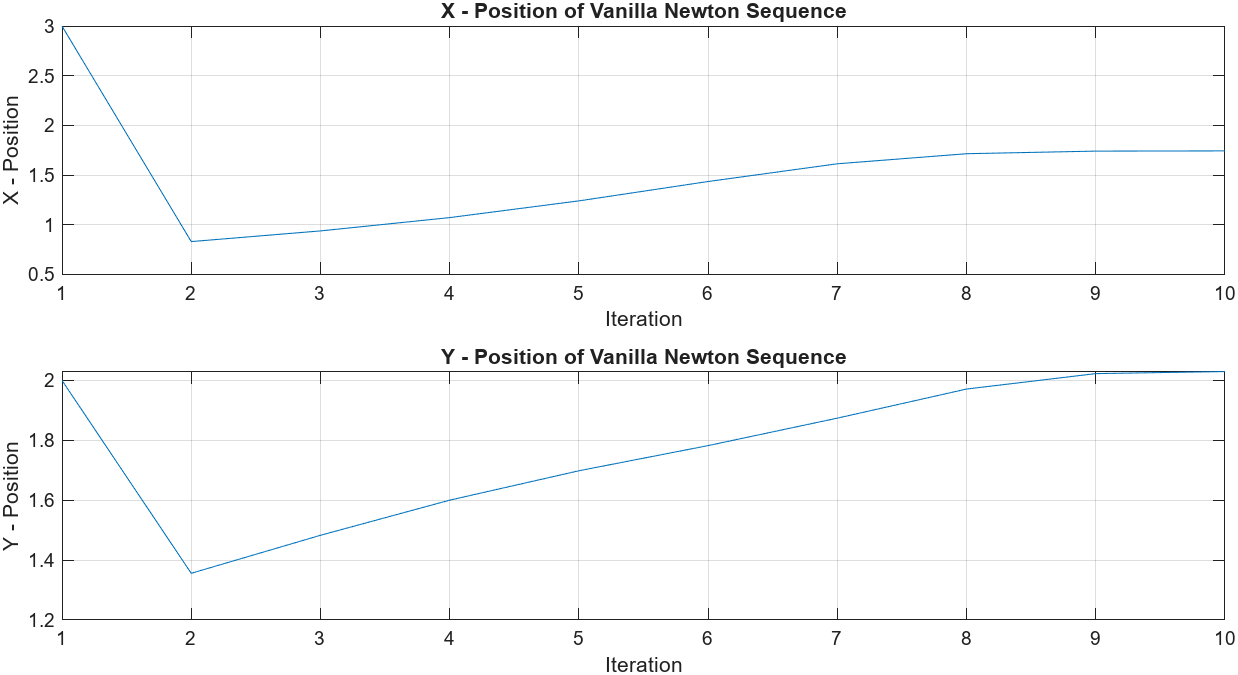
\includegraphics[width=\linewidth]{Images/Fenton_32_VN.png}
    \caption{Sequence for Vanilla Newton at initial condition [3, 2].}
    \label{fig:VN4}
  \end{minipage}\hfill
  \begin{minipage}{0.45\textwidth}
    \centering
    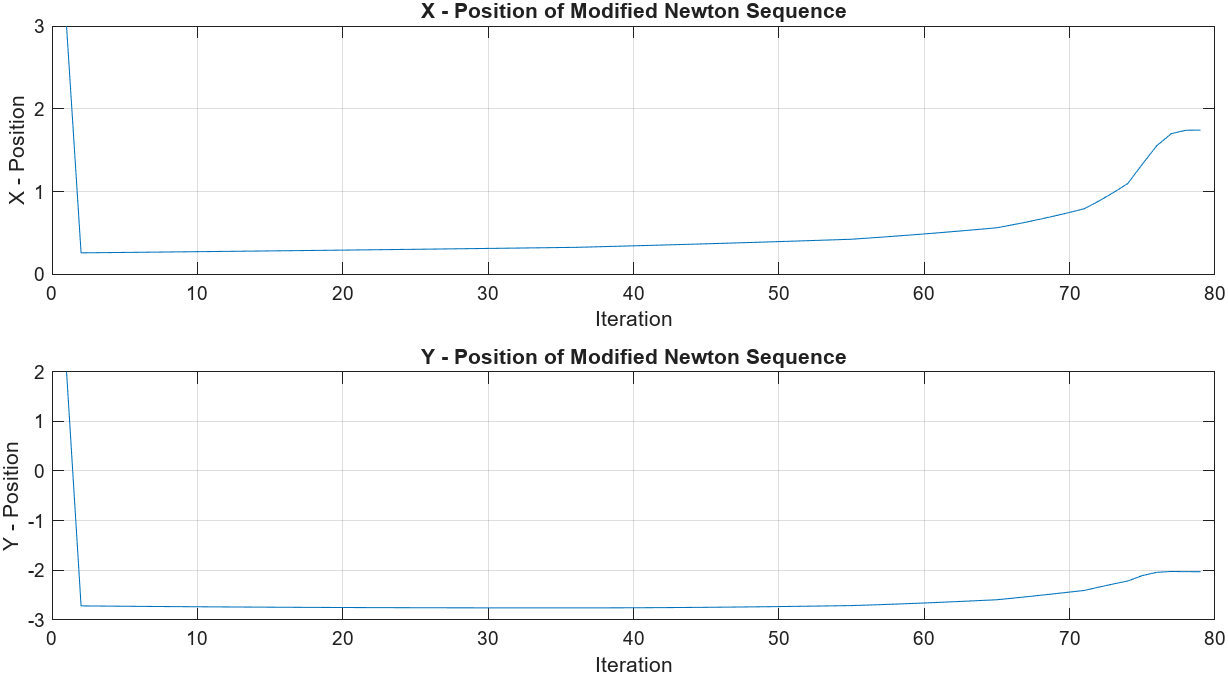
\includegraphics[width=\linewidth]{Images/Fenton_32_NMHM.png}
    \caption{Sequence for Modified Newton at initial condition [3, 2].}
    \label{fig:NMHM4}
  \end{minipage}
\end{figure*}

\vspace{1cm}
\begin{figure}[!ht]
    \centering
    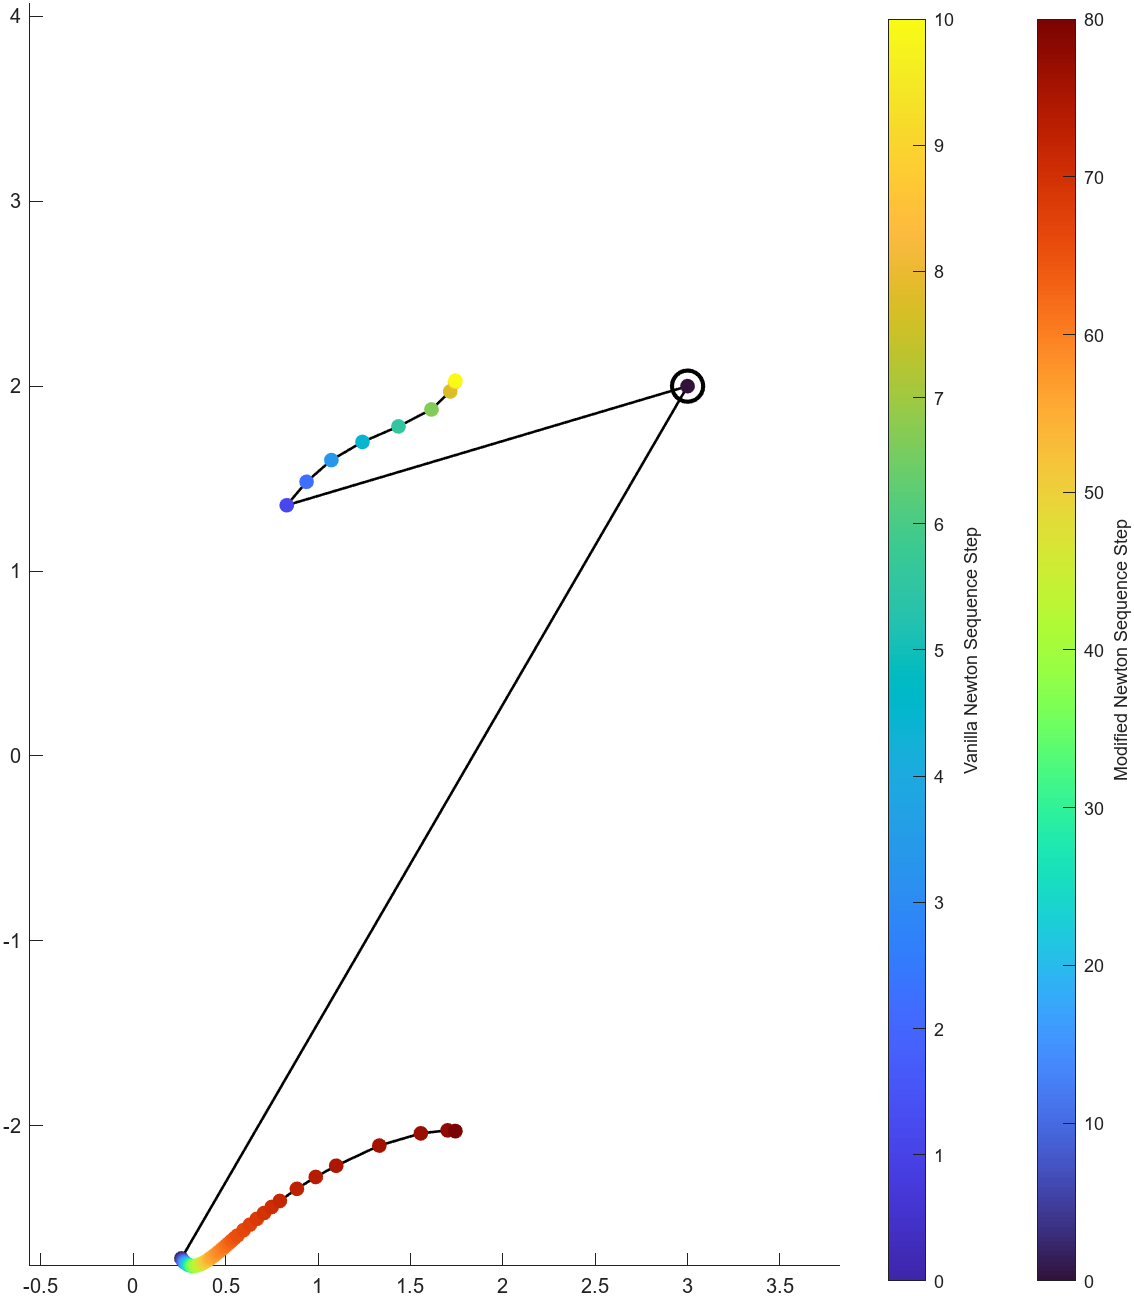
\includegraphics[width = 0.5\textwidth]{Images/Fenton_32_total.png}
    \caption{Sequences for Vanilla Newton and Modified Newton compared for initial condition [3, 2]. The legend is indicated as the different colormaps. The initial point is also circled. }
    \label{fig:total4}
\end{figure}

\clearpage

\begin{figure*}[!htb]
  \centering
  \begin{minipage}{0.45\textwidth}
    \centering
    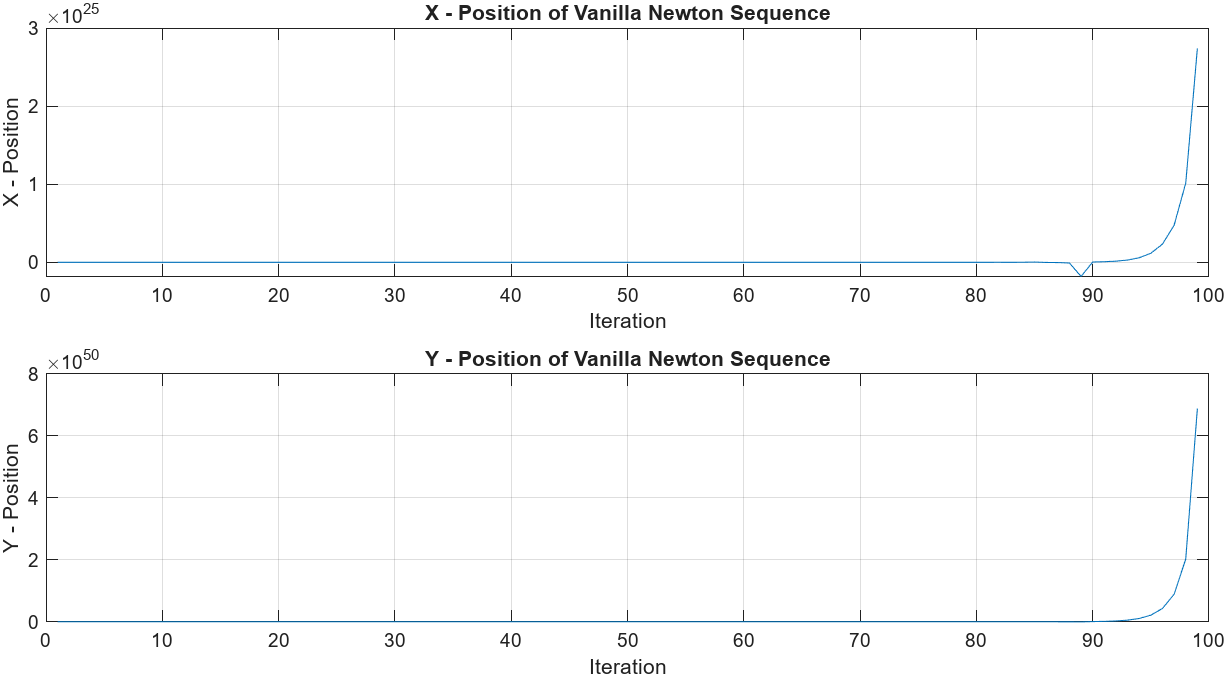
\includegraphics[width=\linewidth]{Images/Fenton_34_VN.png}
    \caption{Sequence for Vanilla Newton at initial condition [3, 4].}
    \label{fig:VN42}
  \end{minipage}\hfill
  \begin{minipage}{0.45\textwidth}
    \centering
    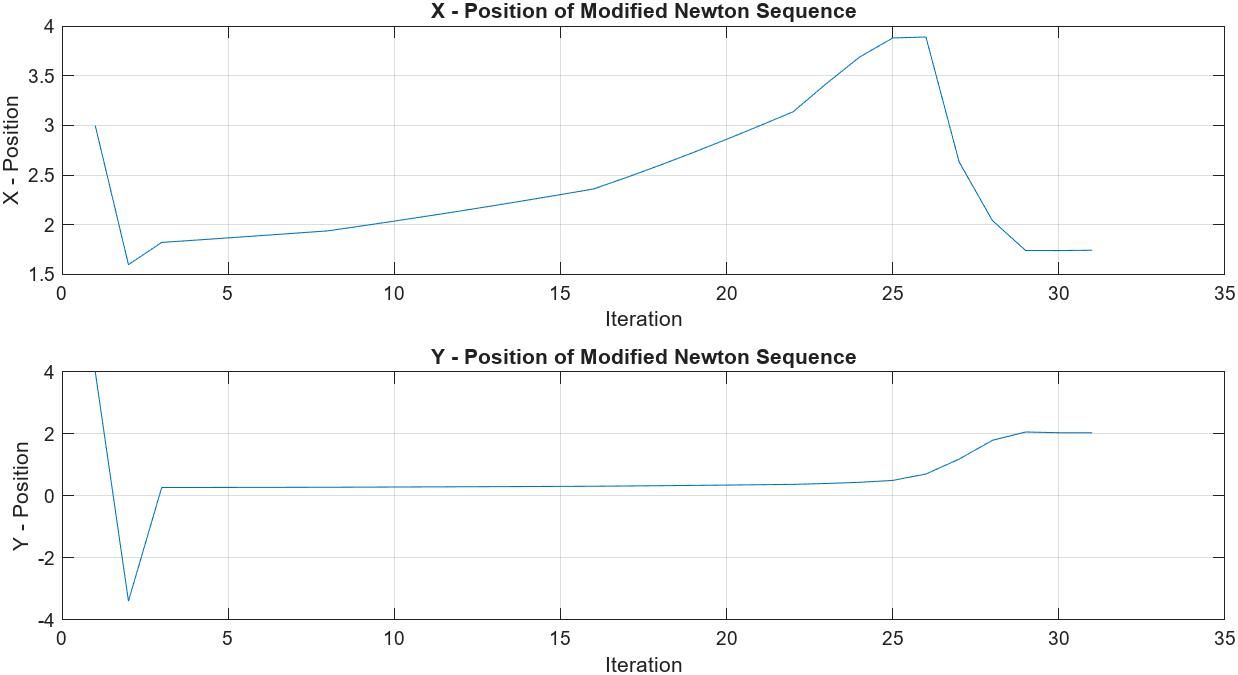
\includegraphics[width=\linewidth]{Images/Fenton_34_NMHM.png}
    \caption{Sequence for Modified Newton at initial condition [3, 4].}
    \label{fig:NMHM42}
  \end{minipage}
\end{figure*}
\vspace{1cm}
\begin{figure}[!ht]
    \centering
    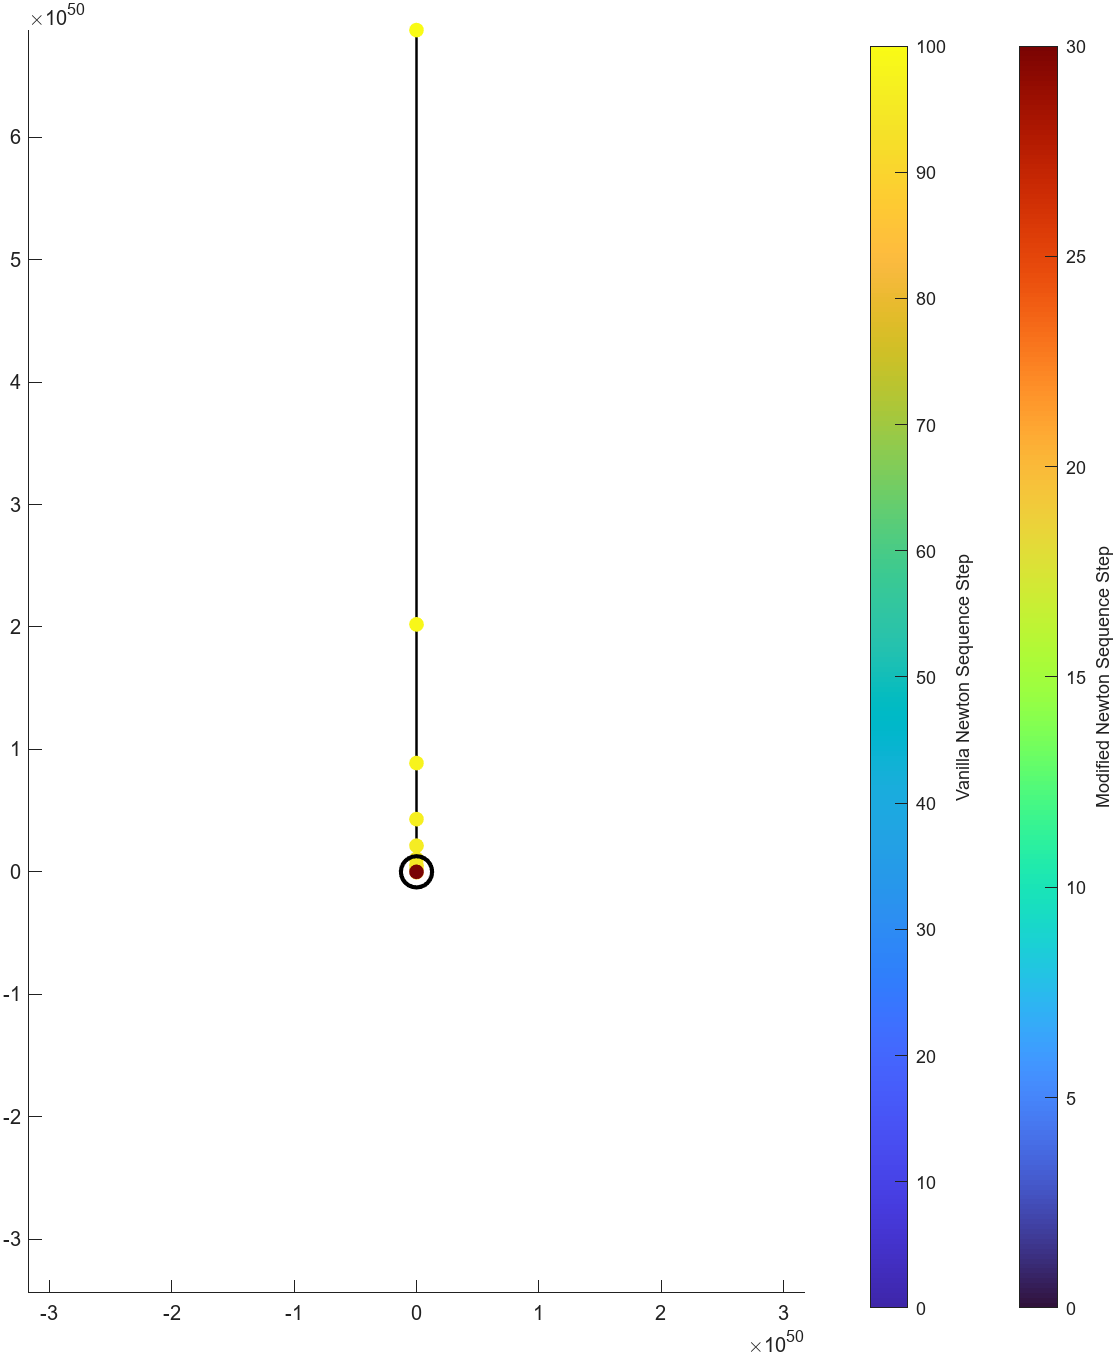
\includegraphics[width = 0.5\textwidth]{Images/Fenton_34_total.png}
    \caption{Sequences for Vanilla Newton and Modified Newton compared for initial condition [3, 4]. The legend is indicated as the different colormaps. The initial point is also circled. }
    \label{fig:total42}
\end{figure}

\newpage
\subsection{Problem 3, part 5}
Apply both methods to the order n Rosenbrock function\\
$f(x) = \sum_{i = 1}^{n - 1} \left [ 100 ( x_{i+1} - x_i^2)^2 + (x_i - 1)^2\right]$\\
starting from the point with all entries equal to 5 and then all entries equal to 10, for increasing $n$. You can tell by inspection that its minimum has all entries equal to 1, but its Hessian is quite degenerate at the solution. This is meant to show what you can expect if the second order sufficient conditions almost do not hold. \\
If you code the derivatives by hand, then implement the function (in Matlab) [f, g, H] = rosenbrockfgH(x), where x is  the evaluation point of function, gradient, and Hessian evaluation. Use the gradient norm less than 1e-3 ...1e-6 as a stopping criterion. For the entry of all 10s, plot the compute times on your computer as a function of n (take n up to a point where the total time of one run does not exceed 1 minute or something you can tolerate). Describe anything you observe that you may not have expected. 
\partbreak
\begin{solution}

    I have included the plots for $x0 = [10]^n$, i.e. the initial point begins at $x_0^{(i)} = 10$ for all $i \leq n$, below. Note that I only went up to 1 minute for both tests. Note that not only did I have a stopping criterion for the normed gradient to be less than some epsilon, I also had a max iteration amount of 1000, just so we don't get hung up on diverging sequences. We would also notice the divergence on the timed figures, since they would deviate quite heavily from the expected characteristic of the graph. This can be seen quite frequently, actually. Notice that Vanilla Newton, Figure \ref{fig:VNTime}, took pretty much linear time in computation. This is very surprising to me at first, due to the nature of linear algebra, I would have expected it to be of order $n^2$. I let the modified Newton run for 10 minutes, to see its shape. It turns out that it is also linear, another surprise.  
\end{solution}

\begin{figure*}[!htb]
  \centering
  \begin{minipage}{0.45\textwidth}
    \centering
    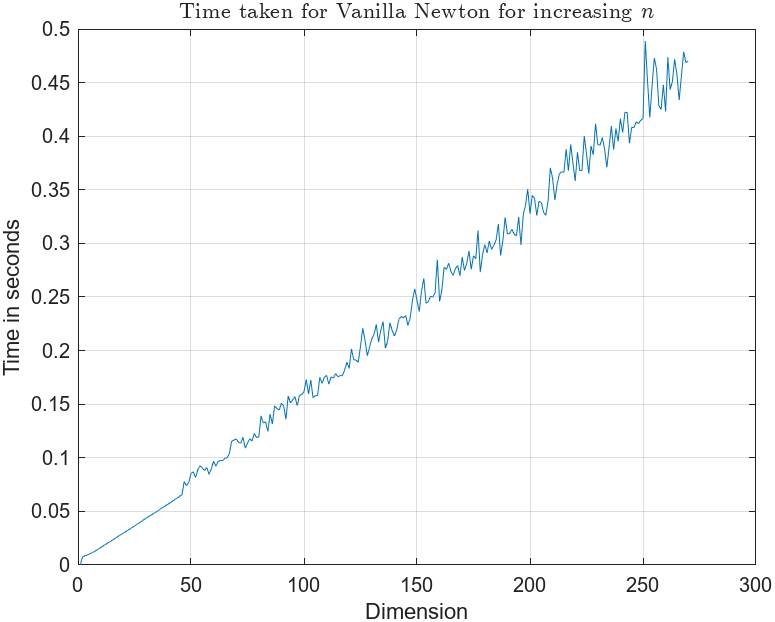
\includegraphics[width=\linewidth]{Images/VN_time.png}
    \caption{Time taken for Vanilla Newton to stop on order $n$ Rosenbrock function for increasing $n$.}
    \label{fig:VNTime}
  \end{minipage}\hfill
  \begin{minipage}{0.45\textwidth}
    \centering
    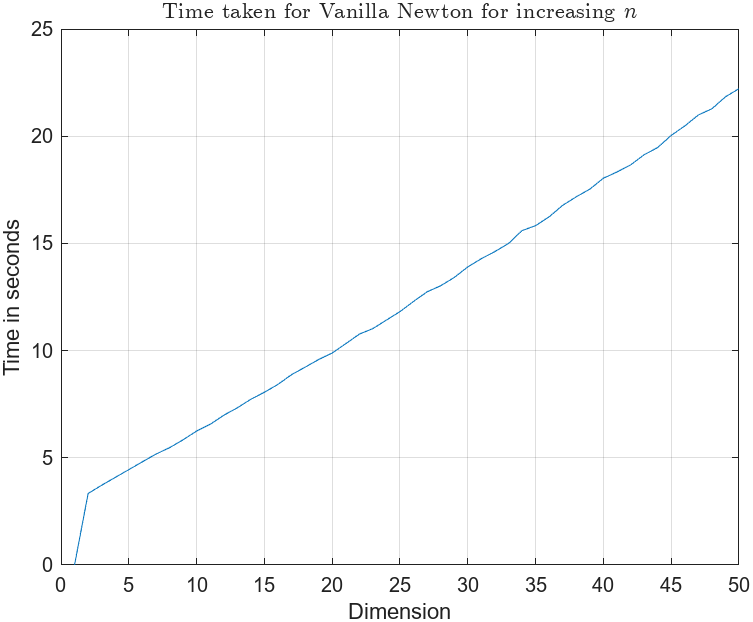
\includegraphics[width=\linewidth]{Images/NMHM_time.png}
    \caption{Time taken for Modified Newton to stop on order $n$ Rosenbrock function for increasing $n$. The plot title is incorrect.}
    \label{fig:NMHMTime}
  \end{minipage}
\end{figure*}
\end{document}